\section{Publish/Subscribe-Systeme}
\label{chap:grundlagen:pubsub}
Publish/Subscribe-Systeme sind Forschungszweck vieler wissenschaftlicher Arbeiten (z.B. \cite{Banerjee2001Comparative, Liu2003Survey, Muhl2002LargeScale, FiegeSecurity, Castro2002Scribe}) und daher gut erforscht und beschrieben. Diese Systeme eigenen sich auf Grund ihres Aufbaus sehr gut zur Eventverteilung in dezentralen Systemen, da sie gegenüber anderen Nachrichtensystemen (wie z.B. \emph{message passing} oder \emph{rpc}) in drei orthogonalen Dimensionen skalieren \cite{PatrickTh2003Many}.

\begin{figure}[htbp]
\centering
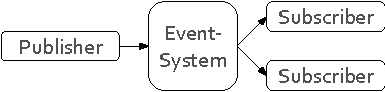
\includegraphics{grafics/pubsub_black_box.pdf}
\caption{Schema eines Publish/Subscribe-Systemes.}
\label{fig:pubsub_black_box}
\end{figure}

\paragraph{räumliche Trennung}
Wie in \Fref{fig:pubsub_black_box} zu sehen ist, trennt das Event-System Publisher und Subscriber räumlich voneinander. Diese Trennung bezieht sich nicht alleine auf verschiedene Schichten einer eine Applikation, sondern kann auch über Applikationsgrenzen oder gar Rechnergrenzen gehen.\\
Weiterhin skaliert ein solches System besser, da der Publisher nur mit dem Event-System kommuniziert und dieses darauf ausgelegt ist, viele Subscribern zu bedienen.

\cite{PiEyKoSh2007-PubSubAPI} gibt einen Vorschlag für eine generische API für Publish/Subscribe-Systeme und unterteilt die Kompabilität verschiedener Systeme in drei Level. Das höchste Level beschreibt einen Datenaustausch der an XML-RPC angelegt ist. Implementieren Systeme dieses Level, so können verschiedene Publish/Subscribe-Systeme miteinander kommunizieren.

\paragraph{zeitliche Trennung}
Publisher und Subscriber sind in ihren Aktionen mit dem Event-System zeitlich getrennt. Ein Publisher muss kein Wissen über Subscriber haben und umgekehrt. Dies bedeutet dass sich ein Subscriber am System anmelden kann, obwohl kein Publisher vorhanden ist. Für Publisher gilt dies analog. Bei \emph{message-passing} ist dies nicht möglich, da die Gegenseite bekannt sein muss.

\paragraph{asynchrone Verarbeitung}
Das Senden einer Nachricht ist für den Publisher nicht blockierend. Die Auslieferung der Nachricht erfolgt für die Subscriber ebenfalls nicht blockierend, da ihnen die Nachricht per Callback zugestellt wird und damit die Verarbeitung vom Event-System aus gestartet wird.


\subsection{Kanalbasiert}
\label{chap:grundlagen:pubsub:kanalbasiert}
Ein prominenter Vertreter dieser Art ist Scribe \cite{Castro2002Scribe}, dessen Funktionsweise in \Fref{chap:related:scribe} genau beschrieben wird.

\subsection{Filterbasiert}
\label{chap:grundlagen:pubsub:filterbased}
\cite{Bharambe2004Mercury} %mercury
\Fref{chap:related:mercury}

\cite{Demers2006Towards} %Cayuga

\cite{Huebsch2003ContentBased}

%\cite{citeulike:4291} %Cluster

